%%%%%%%%%%%%%%%%%%%%%%%%%%%%%%%%%%%%%%%%%
% Medium Length Professional CV
% LaTeX Template
% Version 2.0 (8/5/13)
%
% This template has been downloaded from:
% http://www.LaTeXTemplates.com
%
% Original author:
% Trey Hunner (http://www.treyhunner.com/)
%
% Important note:
% This template requires the resume.cls file to be in the same directory as the
% .tex file. The resume.cls file provides the resume style used for structuring the
% document.
%
%%%%%%%%%%%%%%%%%%%%%%%%%%%%%%%%%%%%%%%%%

%----------------------------------------------------------------------------------------
%	PACKAGES AND OTHER DOCUMENT CONFIGURATIONS
%----------------------------------------------------------------------------------------

\documentclass{resume} % Use the custom resume.cls style

\usepackage[left=0.75in,top=0.5in,right=0.75in,bottom=0.5in]{geometry} % Document margins
\usepackage{hyperref}
\usepackage{array} 
\usepackage{textpos}
\usepackage[utf8]{inputenc}
\usepackage{graphicx}
\usepackage{enumitem}
\usepackage[russian,english]{babel}
\setcounter{secnumdepth}{4}

\begin{textblock}{7}(0, 0.05)
    {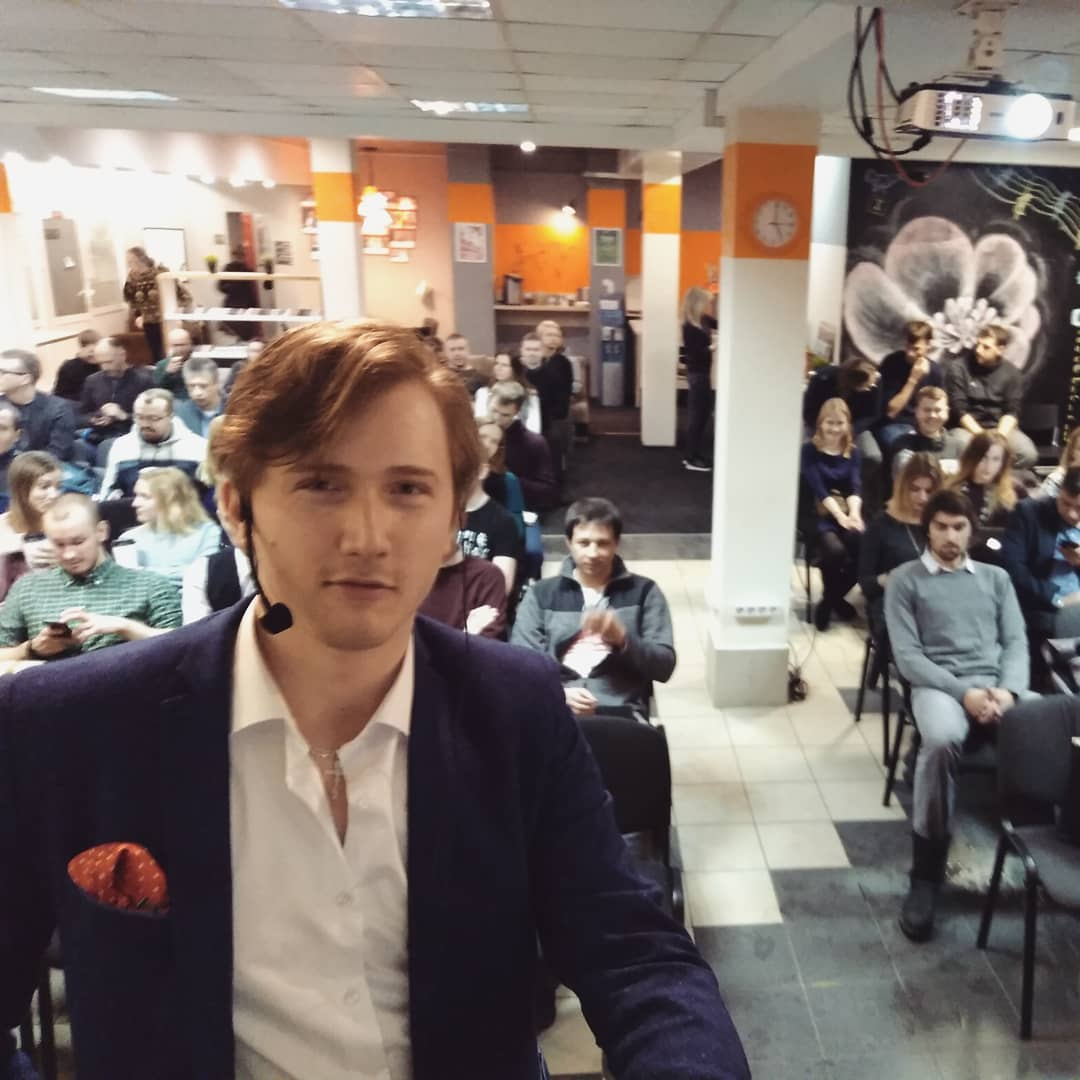
\includegraphics[width=.25\linewidth]{photo.jpg}}
\end{textblock}

\name{Alexander Mikhalchenko} % Your name
\address{Belarus, Minsk 220113} % Your address
\address{\href{http://linkedin.com/in/mikhalchenkoa}{linkedin.com/in/mikhalchenkoa} \\ \href{https://medium.com/@alexandermikhalchenko}{Medium} \\ StackOverflow: \href{http://stackoverflow.com/users/2044039}{id 2044039}} \\
\address{alex@xfuturum.com} % Your phone number and email

\begin{document}

%----------------------------------------------------------------------------------------
%	SUMMARY SECTION
%----------------------------------------------------------------------------------------

\begin{rSection}{Summary}

IT Expert, Senior Fullstack Developer, R\&D engineer, Consultant with extensive experience in Startups.
I am someone who can deliver big things in tight time.
Strong mathematical background, empathic communicator.

\end{rSection}


%----------------------------------------------------------------------------------------
%	TECHNICAL STRENGTHS SECTION
%----------------------------------------------------------------------------------------

\begin{rSection}{Technical Strengths}

\begin{tabular}{ @{} >{\bfseries}l @{\hspace{4ex}} l }
JavaScript  & React, Redux, React Native, Angular, Aurelia, jQuery, D3 \\
NodeJS  & NPM, next.js, Webpack, Express, Grunt, Gulp, Isomorphic apps \\
PHP & PHP7, Symfony, Wordpress, Doctrine, PDO \\
Databases & RabbitMQ, ElasticSearch, MySQL, MongoDB, MapReduce, Redis, SQLite \\
Other & AWS, Python, Groovy, Painless, etc
%VCS & Git, Perforce \\
\end{tabular}

\end{rSection}

%----------------------------------------------------------------------------------------
%	WORK EXPERIENCE SECTION
%----------------------------------------------------------------------------------------

\begin{rSection}{Experience}

\begin{rSubsection}{Xfuturum}{February 2017 - Present}{Founder, Head of Development}{}
\item I manage projects and small dev teams.
\item We primarily work with startups (Series A, B).
\item Full-stack development, Application architecture development, R\&D
\end{rSubsection}


\begin{rSubsection}{Toptal}{February 2017 - Present}{Senior Fullstack Developer, Consultant, NDA-protected}{}
\item IT Consulting
\item Frontend development
\end{rSubsection}


\begin{rSubsection}{TractionBoard}{March 2016 - September 2017}{CTO}{}
\item Architecture development
\item Developing algorithms for BigData processing (RabbitMQ, Mongo, ElasticSearch Groovy scripting)
\item BigData processing (ElasticSearch Scripting - Groovy) and visualization (D3)
\end{rSubsection}

\begin{rSubsection}{Jooicer}{Feb 2017 - September 2017}{CTO}{}
\item A side-project of Tractionboard
\item Developed Twitter automation tools including custom PhantomJS-based scripts
\end{rSubsection}

\begin{rSubsection}{Severex / Pegasus.ae}{November 2015 - December 2016}{Senior Frontend Developer (Aurelia)}{}
\item Working on Aurelia-based frontend, BigData visualization, R\&D
\item Creating prototypes and proof-of-concepts for exhibitions including Abu Dhabi Smart City conference 
\end{rSubsection}

\begin{rSubsection}{DualLab}{August 2015 - December 2015}{Full-stack Web Developer}{}
\item Single-handedly developed the backend (Node.js, TDD)
\item Actively participated in frontend development (Angular)
\end{rSubsection}

\clearpage
%------------------------------------------------


\begin{rSubsection}{StarOfService}{April 2014 - August 2015}{Full-stack Web Developer}{}
\item Worked both on backend (PHP, Symfony 1.4), REST API for apps and frontend (Angular)
\item AWS integration (SQS, S3 integration)
\item Single-handedly developed and maintained primary search engine (TF-IDF based)
\end{rSubsection}


\begin{rSubsection}{Athena Art}{February 2014 - January 2016}{Wordpress Developer, Consultant}{}
\item Did lots of Wordpress customization
\item Site speed and Caching enchantments (from 1.5s to 30ms for homepage)
\end{rSubsection}

\begin{rSubsection}{Itransition}{October 2013 - January 2014}{Fullstack Web developer intern (PHP, C\#)}{}
\end{rSubsection}

%------------------------------------------------

%\begin{rSubsection}{Personal projects}{}{}
%
%\begin{itemize}[leftmargin=*,label={$+$}]
%  \item {\bf \href{http://nagibator.xyz}{VOUFF (ex Nagibator)}} \hfill {\em November 2015 - March 2016}  \\
%	Live image tracking and replacement in videos. 2nd prize at Garage
%	48 hackaton (Nov 2015), participated in TechMinsk Accelerator (Feb 2016).
%
%  \item {\bf \href{http://gendalf.tv}{Gendalf TV}} \hfill {\em December 2015 - April 2016}  \\
%	App for sending videos to LG Smart TV, 1st place at LG Hackaton (Dec 2015).
%
%  \item {\bf \href{http://toto.by}{ToTo.by}} \hfill {\em November 2015}  \\
%	Car-related information aggregator for Belarus.
%
%  \item {\bf \href{http://boxinator.xyz}{Boxinator}} \hfill {\em September 2015} \\
%	Cloud-based workflow management system, participant of Minsk FinTech hackaton.
%
%  \item {\bf \href{http://mmopricefinder.com}{MMOPriceFinder.com}} \hfill {\em July 2014} \\
%	WoW, FIFA and other games inner currency rates search.
%
%\end{itemize}
%\end{rSubsection}
\end{rSection}
%----------------------------------------------------------------------------------------

%----------------------------------------------------------------------------------------
%	EDUCATION SECTION
%----------------------------------------------------------------------------------------

\begin{rSection}{Education}
{\bf Belarussian State University, Belarus} \hfill {\em 2017 $-$ 2018} \\
Master Degree in Computer Science

{\bf Belarussian State University, Belarus} \hfill {\em 2012 $-$ 2017} \\
Bachelor Degree in Computer Science, minor in Intelligent Control Systems \hfill {\em avg: 9.2/10}
% Courses taken: Algorithms, Pattern recognition, Natural Text Processing, Calculus, etc.

{\bf Belarussian State University Lyceum, Belarus} \hfill {\em 2010 $-$ 2012} \\
Associate degree in Mathematics \hfill {\em avg: 9.8/10}
\end{rSection}

%----------------------------------------------------------------------------------------
%	Mathematics
%----------------------------------------------------------------------------------------

\begin{rSection}{Honors \& Awards section}

\begin{rSubsection}{International Tournaments of Young Mathematicians}{}{}

\item ITYM 4 $-$ 1st place \& gold medal \hfill July 2012, Paris, France
\item ITYM 6 $-$ 2nd place \& gold medal (team leader) \hfill July 2014, Bremen, Germany

\end{rSubsection}

\begin{rSubsection}{Belarussian Mathematical Olympiads}{}{}

\item 61st BMO $-$ I diploma \hfill  April 2011, Belarus, Gomel
\item 62nd BMO $-$ II diploma \hfill April 2012, Belarus, Gomel
\end{rSubsection}


\begin{rSubsection}{Local Tournaments of Young Mathematicians}{}{}

\item XIV Belarussian TYM $-$ 1st place (team leader) \hfill December 2012, Belarus, Minsk
\item XV Belarussian TYM $-$ 1st place (team leader) \hfill December 2013, Belarus, Minsk
\item 2nd St.Petersburg TYM $-$ 1st place (team leader) \hfill March 2014, Russia, St. Petersburg
\end{rSubsection}

\end{rSection}

\begin{rSection}{Public Speaking & Publications}

    \begin{rSubsection}{Presentations at local meetups}{}{}

    \item Mentor at Imaguru Coding Fest \hfill Imsguru Startup Hub, Aug 2017
    \item Speaker \hfill Imaguru Project Management Meetup Series
    \item Speaker \hfill Deti MBA, Apr 2018 - Present
    \item Interracting with websites w/o API \hfill WebNotBombs conf, Minsk, Feb 2016
    \item Aurelia vs Angular 2 \hfill The Rolling Scopes \#21, Minsk, Dec 2015


    \end{rSubsection}

    \begin{rSubsection}{Publications}{}{}

    \item Sentimental corpus \& Semantic Web problems in tourism domain \hfill 72nd BSU Scientific Conference
    \item Plant Phenomics and Image processing Algorithms \hfill 73rd BSU Scientific Conference
    % ("Система синтеза сентиментального корпуса текста для решения задач semantic web в области туризма")%.
    \item Decision support systems and plant phenomics \hfill PRIP'16
    \item \href{http://textlab.io/doc/8452214}{Designing the platform for phenotyping stem cuttings and clones of ornamental woody plants}
    \end{rSubsection}
\end{rSection}


%----------------------------------------------------------------------------------------
%	EXAMPLE SECTION
%----------------------------------------------------------------------------------------

%\begin{rSection}{Section Name}

%Section content\ldots

%\end{rSection}

%----------------------------------------------------------------------------------------

\end{document}
